\documentclass[pdflatex,sn-basic]{sn-jnl}

\usepackage{graphicx}
\graphicspath{{./}{../figures_pdf_vector/}}
\usepackage{multirow}
\usepackage{amsmath,amssymb,amsfonts}
\usepackage{amsthm}
\usepackage{mathrsfs}
\usepackage{xcolor}
\usepackage{textcomp}
\usepackage{manyfoot}
\usepackage{booktabs}
\usepackage{listings}
\usepackage{array}

\raggedbottom

\begin{document}

\title{Online Resource 1: Operational Characterisation of the Primary Subject}

\author*[1]{\fnm{Shweta} \sur{Mishra}}\email{shweta.mishra.research@gmail.com}

\affil*[1]{\orgname{Independent Researcher}, \orgaddress{\city{Moradabad}, \country{India}}}

\abstract{Supplementary material accompanying ``Boundary-Mutation Testing for Pattern-Based Secret Detection: A Rule-Level Method and Cross-Scanner Evaluation.'' This resource reports the operational behaviour of the primary subject's ingress pipeline, event queue, worker pool and fault tolerance. None of it is evidence for or against any claim in the main paper.}

\maketitle

This document reports the operational behaviour of the primary subject: its ingress pipeline, event queue, worker pool and fault tolerance. \textbf{None of it is evidence for or against any claim in the main paper.} It is included for two reasons. First, a reader assessing whether a defect in this scanner is worth attending to is entitled to know whether the surrounding system is a maintained service or a prototype. Second, the measurements exist, were produced by the same pinned harness, and withholding them from a paper that argues for reporting inconvenient evidence would be inconsistent.

The unit of analysis in the main paper is a detection rule; here it is a running service. That is a different artefact, which is why this material is reported as a separate online resource and not as a research question.

\section{Concurrency and latency}

Fig.~\ref{fig:scaling} gives throughput and tail latency for the circuit breaker from 1 to 128 threads, and Fig.~\ref{fig:payload} the ingress pipeline latency against payload size. Each thread performs a fixed 1{,}500 operations, so offered load grows with thread count; threads are released by a \texttt{threading.Barrier} so that timing begins only once every thread is running. Each level is repeated 7 times and reported with the 95\% confidence interval of the mean.

The barrier matters, and its absence is the second harness defect we disclose. An earlier version started threads without synchronisation; at high thread counts the first threads finished before the last had started, and the resulting curve showed throughput \emph{rising} with contention. That curve was an artefact of the harness, not a property of the system. We report it because it is the more instructive of our two mistakes: it produced a plausible, publishable-looking result that was entirely wrong.

Scanner throughput over 30 repetitions of 2{,}000 scans has a median of 11{,}114 scans/s (mean 11{,}104, sd 123), which is the basis for the claim in the main paper that the mutation battery is cheap to run.

\begin{figure}[t]
\centering
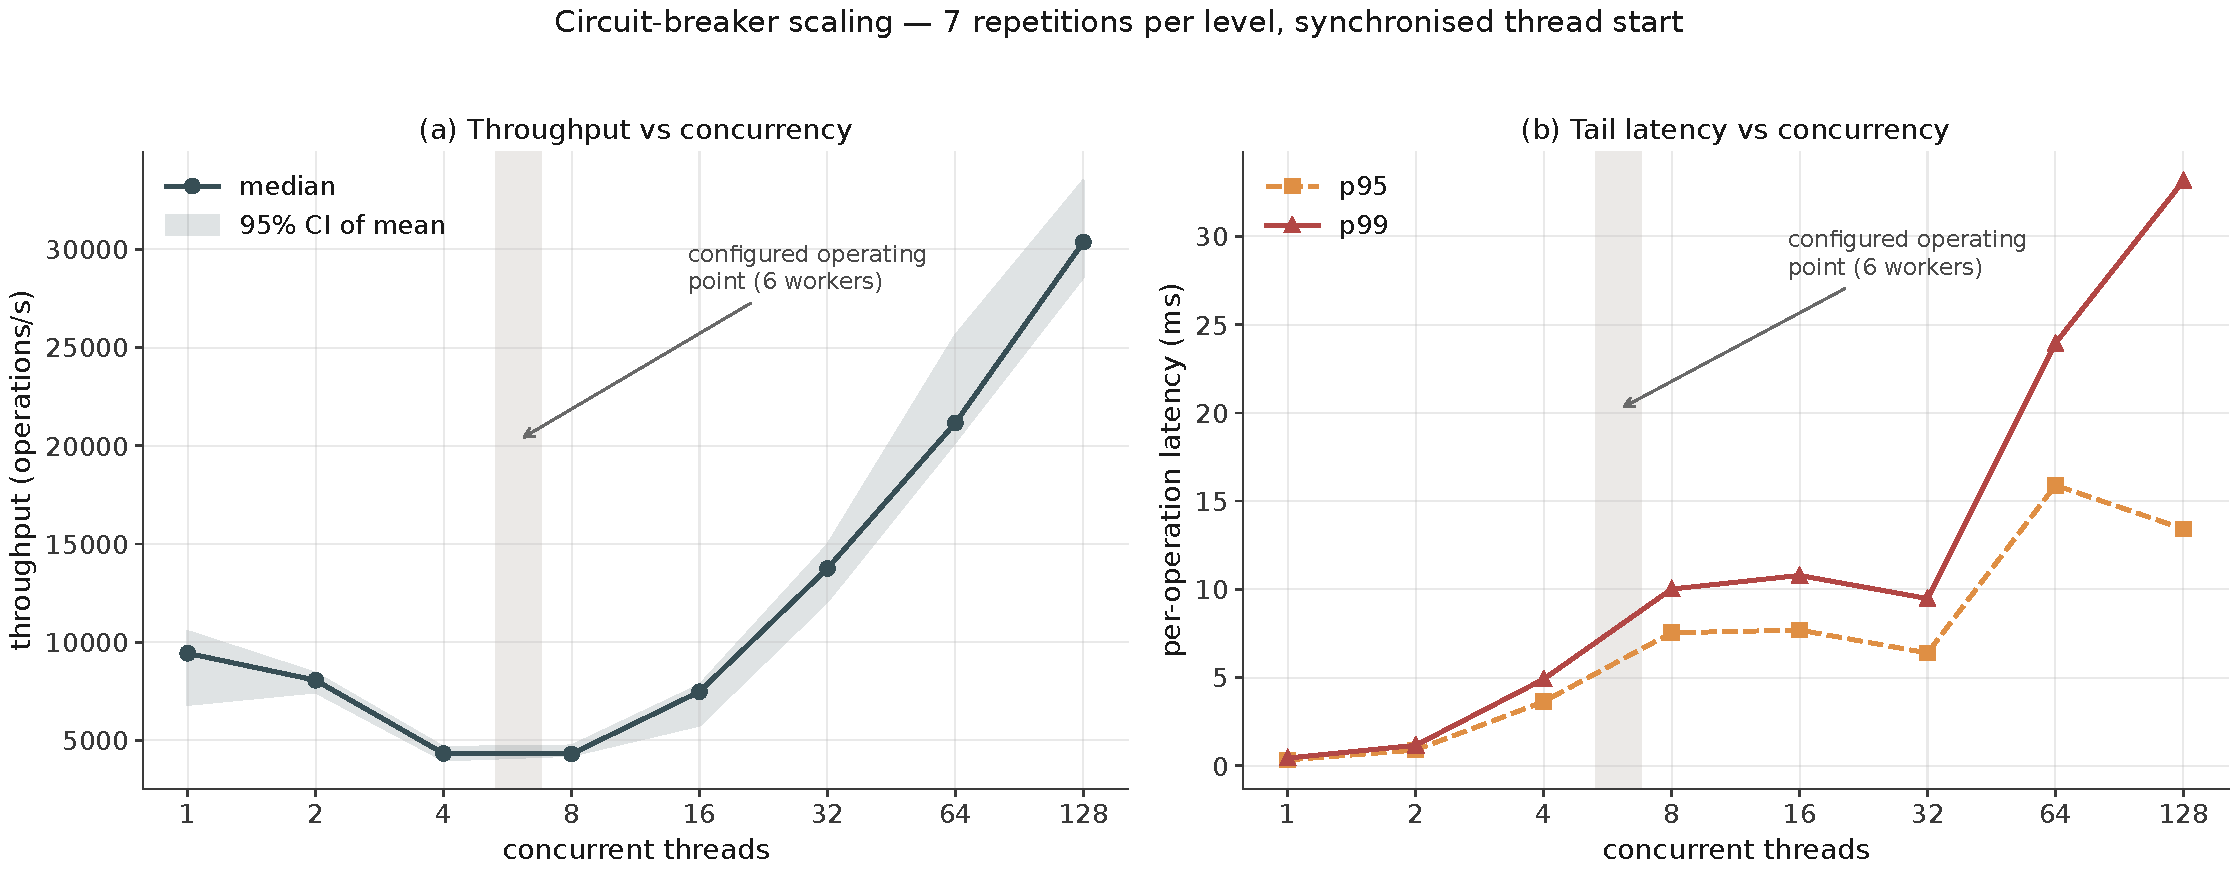
\includegraphics[width=0.92\textwidth]{fig09_scaling.pdf}
\caption{Circuit-breaker throughput and tail latency, 1--128 threads, synchronised start, 7 repetitions per level.}
\label{fig:scaling}
\end{figure}

\begin{figure}[t]
\centering
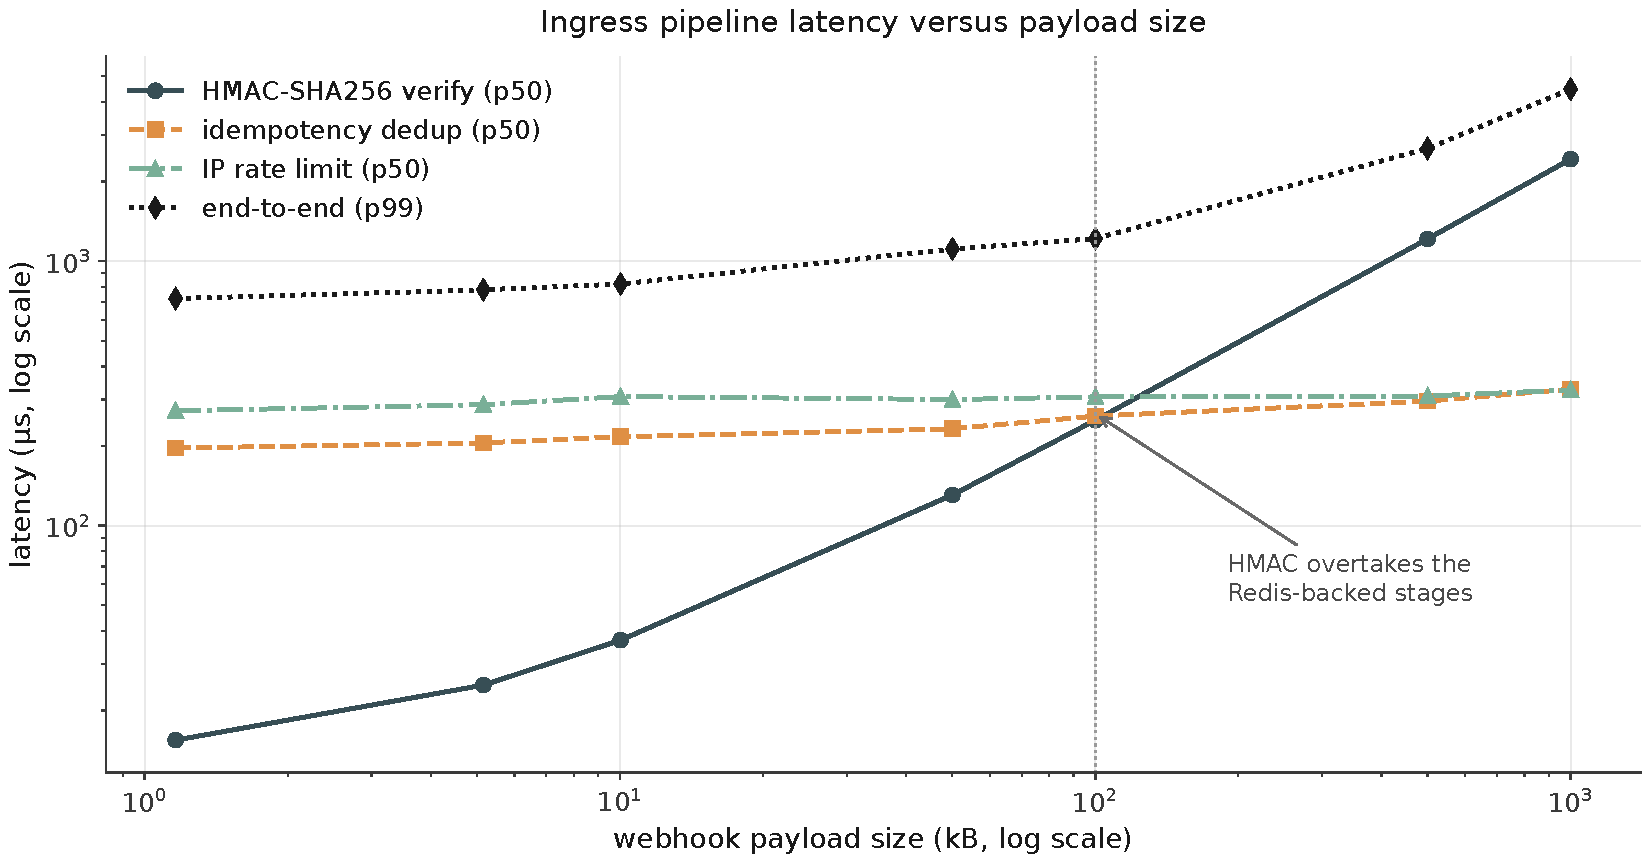
\includegraphics[width=0.92\textwidth]{fig10_payload.pdf}
\caption{Ingress pipeline latency against payload size, 400 trials per repetition, 5 repetitions.}
\label{fig:payload}
\end{figure}

\section{Fault injection}

Table~\ref{tab:faults} and Fig.~\ref{fig:faults} report four injected faults. All measurements use unmodified production modules against a real \texttt{redis-server} 7.0.15 on loopback with persistence disabled; the loopback configuration makes every latency figure a lower bound.

\begin{table}[t]
\centering
\caption{Fault injection. All four oracles hold.}
\label{tab:faults}
\footnotesize
\setlength{\tabcolsep}{3pt}
\begin{tabular}{@{}p{2.25cm}p{2.75cm}r@{}}
\toprule
Fault & Oracle & Result \\
\midrule
\multirow{2}{=}{Redis killed mid-run}
 & uncaught exceptions & 0 of 300 \\
 & degraded gracefully & 180 of 180 \\
\midrule
Redis unavailable & in-memory dedup preserved & holds \\
\midrule
Duplicate delivery & exactly-once & 1 of 10 \\
\midrule
Arrival storm & cap never exceeded & 200 of 1{,}000 \\
\botrule
\end{tabular}
\end{table}

\begin{figure}[t]
\centering
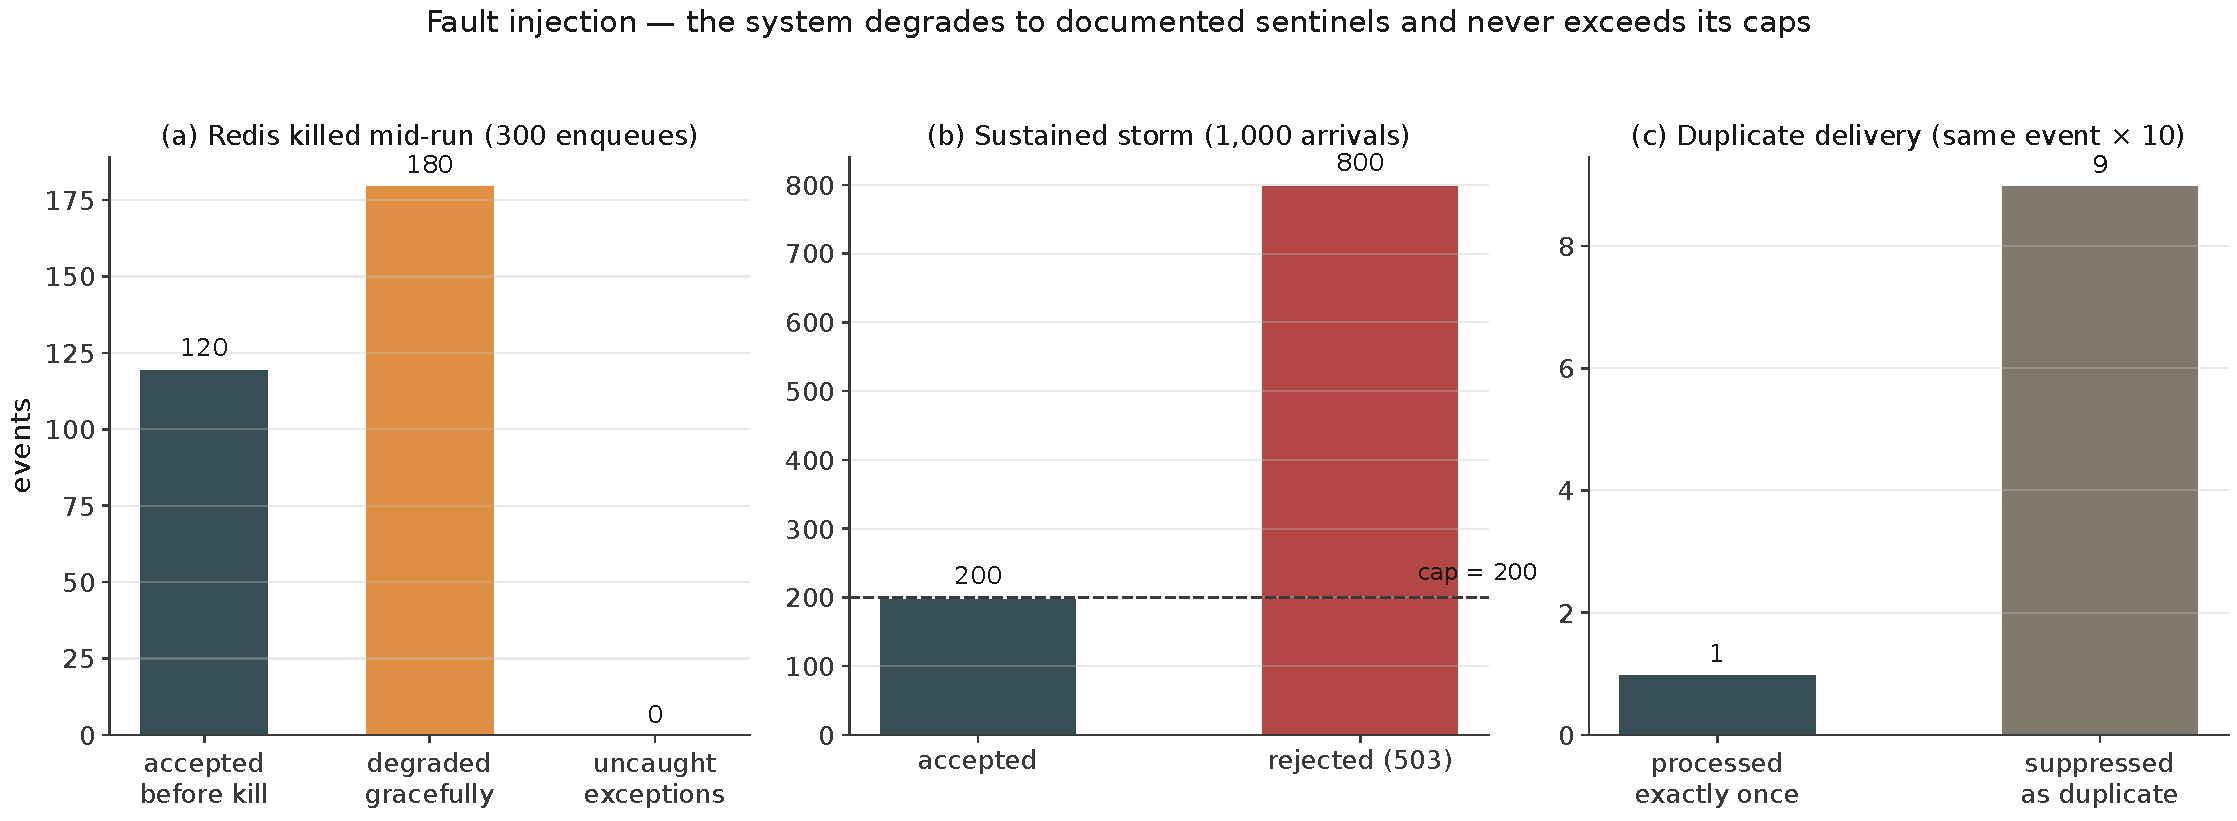
\includegraphics[width=0.92\textwidth]{fig11_faults.pdf}
\caption{Fault injection: Redis termination, dedup fallback, duplicate-delivery suppression, and arrival-storm capping.}
\label{fig:faults}
\end{figure}

When Redis is terminated mid-run, \texttt{enqueue()} returns a sentinel rather than raising, so the caller falls back to direct dispatch: 120 events were accepted before the kill and the remaining 180 degraded without a single uncaught exception. Idempotency survives the loss of Redis through an in-memory fallback. Ten deliveries of one event yield exactly one processed and nine suppressed. Under a 1{,}000-event arrival storm against a queue capped at 200, exactly 200 are accepted and 800 rejected, with the cap never exceeded.

\section{Test suite and complexity}

Fig.~\ref{fig:quality} shows coverage by package and the cyclomatic-complexity distribution; the headline figures appear in the main paper's subject-characteristics table. The distribution is unremarkable --- mean complexity 4.67 over 617 functions --- with a single outlier at 34. We report it for completeness and draw no conclusion from it: nothing in the main paper depends on the subject's internal complexity, and the five defective rules are declarative table entries rather than control flow.

\begin{figure}[t]
\centering
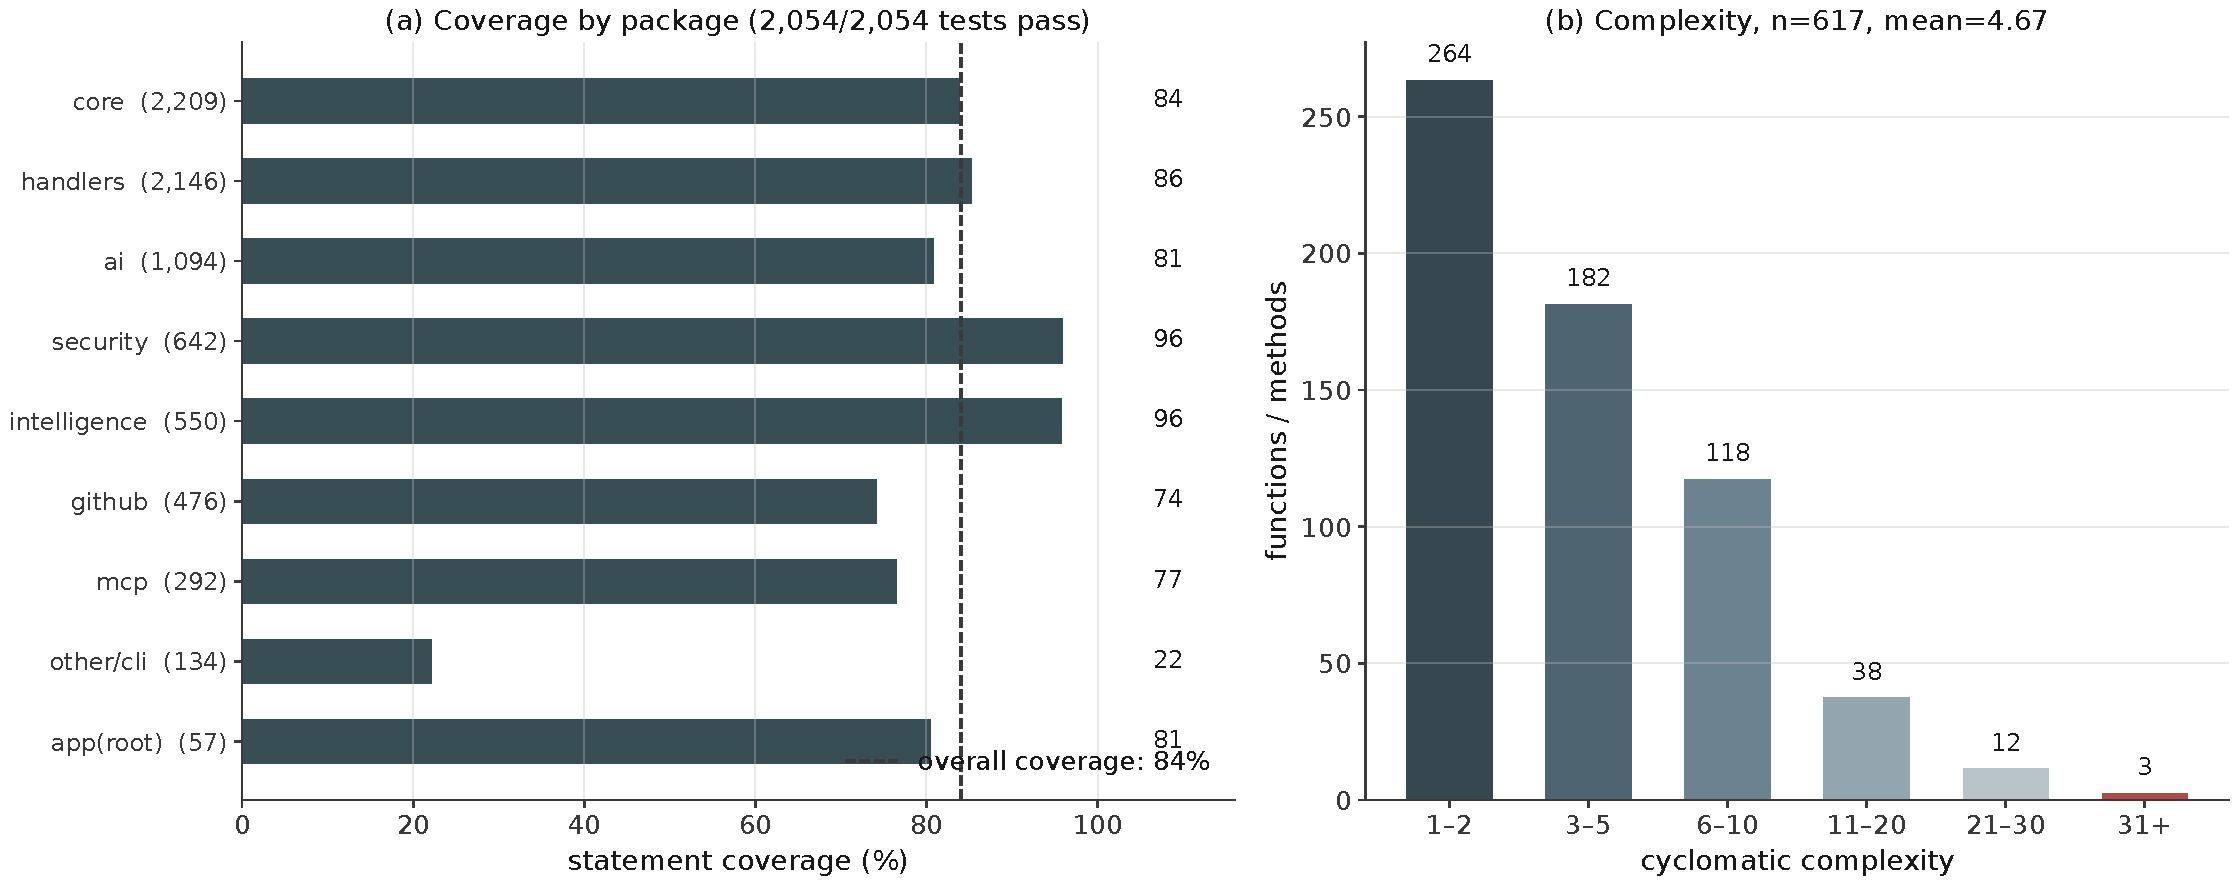
\includegraphics[width=0.92\textwidth]{fig12_quality.pdf}
\caption{Statement coverage by package and cyclomatic-complexity distribution for the primary subject.}
\label{fig:quality}
\end{figure}

\end{document}
